\chapter{La web interactiva}\label{cap:web}

\section{Propósito}

Los algoritmos del viajante son más fáciles de entender viéndolos funcionar que leyendo su pseudocódigo. Por eso, además del estudio, se ha construido una \textbf{web interactiva} que anima los ocho algoritmos sobre el mapa de España, con la ruta construyéndose
paso a paso sobre las carreteras reales. Sirve como apoyo visual para la presentación del trabajo y puede quedar publicada de forma permanente.

\section{Qué ofrece}

La web tiene tres vistas:
\begin{description}[leftmargin=0pt,labelindent=0pt,style=nextline]
  \item[Laboratorio.] Se elige un algoritmo, un conjunto de ciudades (pulsando sobre el mapa o la lista, o con ejemplos predefinidos de 6, 9, 13, 47 y 75 ciudades), la medida (kilómetros o tiempo) y si se respetan los sentidos únicos. Un reproductor permite ejecutar, pausar, avanzar y retroceder
        paso a paso, saltar al resultado final y cambiar la velocidad. Junto al mapa aparecen el \textbf{pseudocódigo con la línea actual resaltada}, una \textbf{explicación en lenguaje llano} de lo que ocurre en cada paso, el coste de la ruta actual y de la mejor encontrada, una gráfica de la evolución del coste y la ficha del algoritmo.
  \item[Carrera.] Varios algoritmos resuelven \emph{a la vez} las mismas ciudades. Cada uno avanza durante el mismo tiempo de cálculo, de modo que el que termina antes es de verdad el más rápido. Al final aparece una tabla con el coste, la desviación frente al mejor y el tiempo de cálculo.
        Los algoritmos no aplicables se descartan con su motivo, igual que en el estudio.
  \item[Acerca de.] Explica qué es la web y cómo se usa.
\end{description}
Hay tema oscuro (mapa nocturno, pensado para proyector) y claro, botón de pantalla completa, zoom con la rueda del ratón y atajos de teclado.

\begin{figure}[htbp]
  \centering
  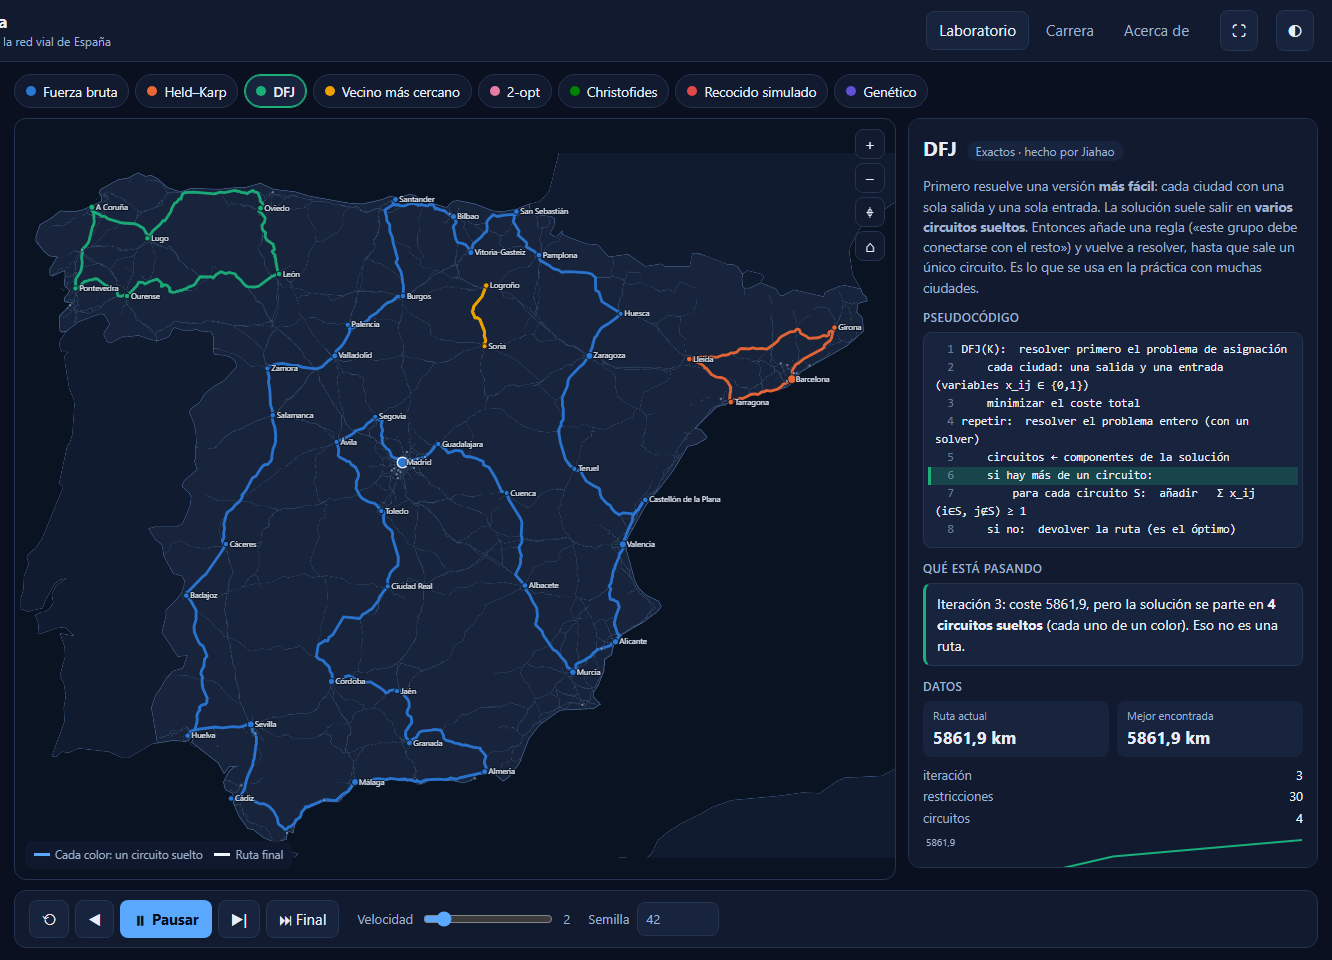
\includegraphics[width=0.97\linewidth]{web_05_dfj_circuitos_sueltos.png}
  \caption{Laboratorio: DFJ con las 47 capitales. La primera solución del problema de asignación se parte en varios circuitos sueltos (cada uno de un color) sobre las carreteras reales; el pseudocódigo resalta el paso actual.}
  \label{fig:web_dfj}
\end{figure}

\begin{figure}[htbp]
  \centering
  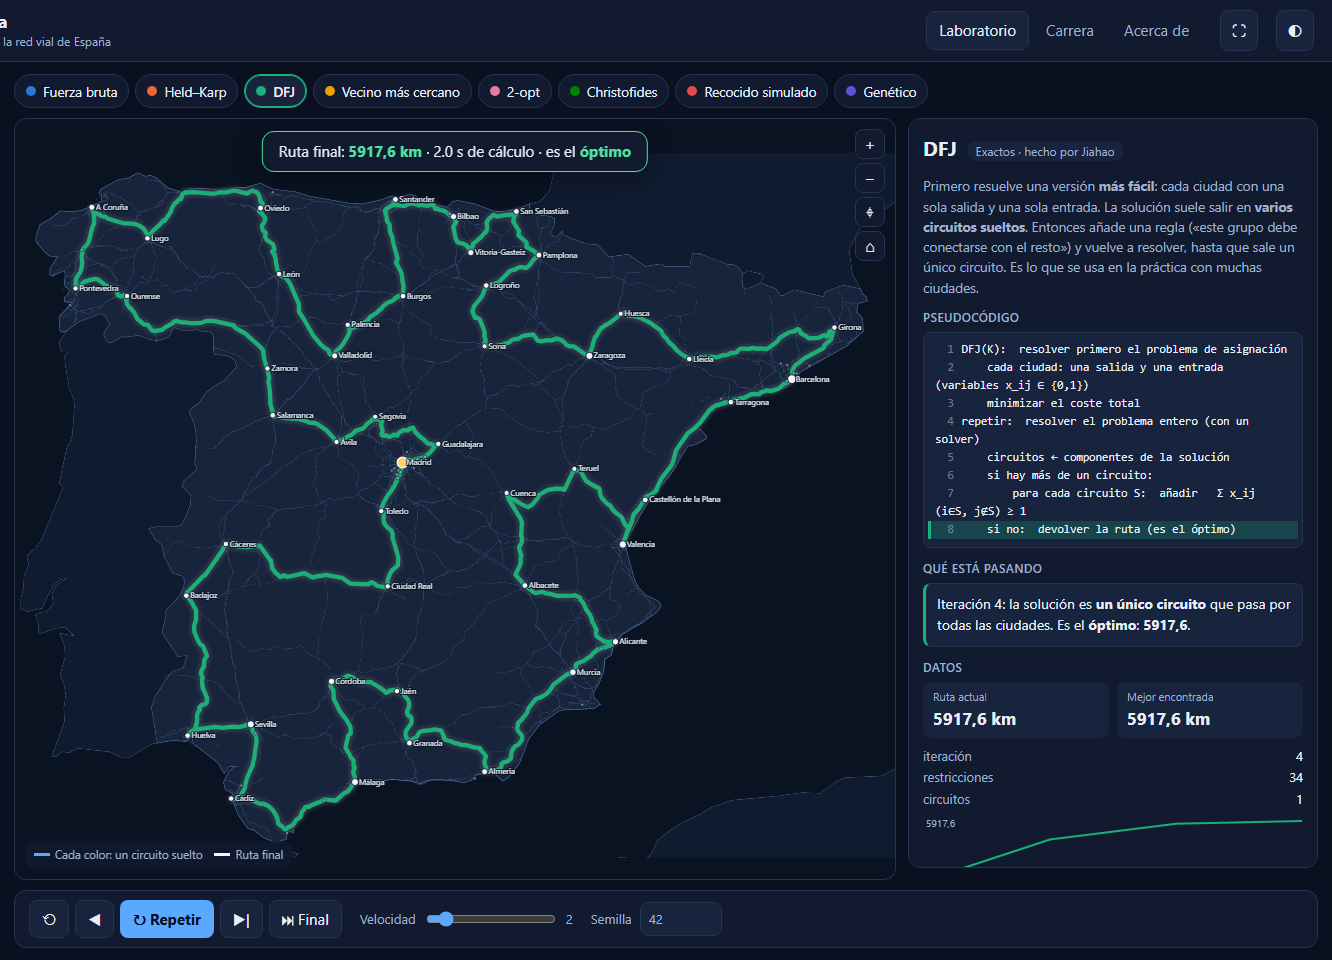
\includegraphics[width=0.97\linewidth]{web_06_dfj_optimo_47_capitales.png}
  \caption{Laboratorio: ruta óptima de las 47 capitales (5.917,6~km) encontrada por DFJ tras cuatro iteraciones.}
  \label{fig:web_optimo}
\end{figure}

\begin{figure}[htbp]
  \centering
  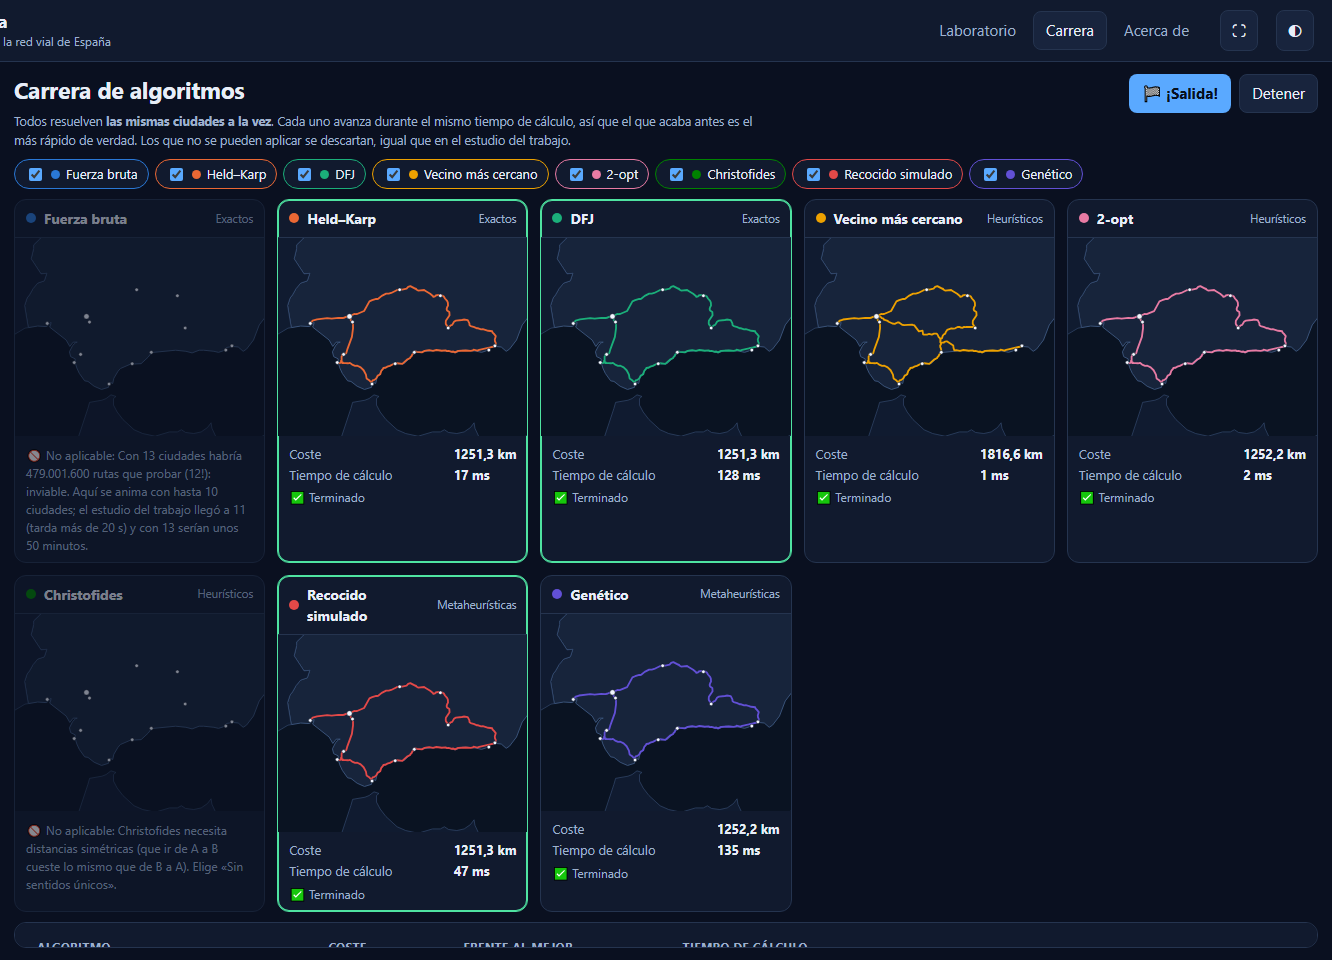
\includegraphics[width=0.97\linewidth]{web_10_carrera.png}
  \caption{Carrera de algoritmos sobre las 13 ciudades de Andalucía. Fuerza bruta y Christofides se descartan con su motivo; Held--Karp, DFJ y el recocido encuentran el óptimo (1.251,3~km) en 17, 128 y 47~ms.}
  \label{fig:web_carrera}
\end{figure}

\section{Cómo está hecha}

\begin{itemize}
  \item \textbf{Sin servidor.} Todo se calcula en el navegador, con JavaScript. Cada algoritmo está escrito como un \emph{generador} en el que cada paso emite un «fotograma» (ruta, aristas resaltadas, línea de pseudocódigo, explicación y coste),
        lo que permite reproducir, pausar y retroceder con el mismo código.
  \item \textbf{Mapa.} Un mapa esquemático propio (contorno de la península y países vecinos, y red de autovías y vías rápidas de fondo) dibujado con \emph{canvas} y SVG, con zoom y desplazamiento.
  \item \textbf{Carreteras reales.} Para cada par de las 75 ciudades se ha precalculado, con el grafo del trabajo, el camino mínimo y se ha guardado su trazado simplificado y codificado (1,1~MB para 2.775 pares); las rutas se dibujan siguiendo esas carreteras.
  \item \textbf{Solucionadores.} DFJ usa \emph{HiGHS}~\cite{huangfu2018}, un \emph{solver} de programación entera compilado a WebAssembly, y Christofides usa el emparejamiento de Edmonds; ambas librerías (licencia MIT) se incluyen en el repositorio, de modo que la web funciona sin internet.
  \item \textbf{Datos.} Las distancias son las mismas tablas del trabajo (capítulo~\ref{cap:versiones}).
\end{itemize}

\section{Cómo sabemos que es correcta}

Los algoritmos de JavaScript se contrastan automáticamente con los resultados de Python: fuerza bruta, Held--Karp y DFJ dan el mismo óptimo (5.917,562~km con las 47 capitales, 460,438~km en Galicia, 1.251,307~km en Andalucía y 6.146,165~km con las 75 ciudades);
el vecino más cercano y el 2-opt dan los mismos costes que en Python (6.772,1~km y 6.326,0~km con las 47 capitales); y Christofides, el genético y el recocido devuelven rutas válidas con costes dentro de lo esperado. Además se probaron las vistas con un navegador automatizado, sin errores de consola.

\section{Publicación}

La web es una carpeta del repositorio (\texttt{web/}) que se abre en local con un servidor sencillo (doble clic en \texttt{iniciar\_web.bat} o \texttt{python -m http.server}). El repositorio incluye además una acción de GitHub que la publica en \emph{GitHub Pages} cuando
el propietario del repositorio la activa, de modo que queda en una dirección permanente. La guía de uso (documento aparte) explica el manejo paso a paso.
